\section{Measuring similarity using Clone Detection approach}
One of the approaches to detecting similarity in code is the Clone Detection. It is able to find the similarities between the code files and also provide the position of duplicates.

\subsection{Code Detection}
Typically, clone detection is done by comparing the two streams of data and spotting out any identical segments that exists in both of the streams. The comparisons can be based on text, tokens, syntax or structures.
The clone detection steps are as follows [1]:
\begin{itemize}
\item Raw code is fed into the pre-processing stage where it removes uninteresting codes such as embedded code such as SQL queries in a Java file. It determines the comparison unit such as tokens, hash or characters, etc.
\item The processed code is then transformed to the form suitable as input to the actual comparison algorithm. It can tokenize or parse depending on the comparison unit and it removes whitespaces and comments to normalise the code.
\item The transformed code is then fed into a comparison algorithm. It aims to find the longest contiguous sequence of similar units. It outputs a list of matches that were found in the transformed code.
\item It then maps the detected clones back to the source code by their line numbers.
\item Then it can be extracted from the source to be visualised for manual inspection, such as the scatter dot plot.
\item Sometimes, in order to reduce the amount of data, it can return only clone pairs as the result. 
\end{itemize}
\begin{figure} [ht]
\centering
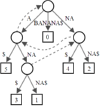
\includegraphics{Figures/clonedetection}
\caption{Clone detection}
\label{fig:clone}
\end{figure}
One of the applications that utilises clone detection is the CCFinder. It aims to be used in an industrial scale and to be applicable to million-line size system. The tool takes token sequences as comparison unit through a lexical analyser and applies rule-based transformation to the sequence, which enables the tool to be able to detect cloned code portions that have different syntax but may have similar meaning. CCFinder utilises suffix tree matching algorithm to detect clones. Suffix tree matching provides the position of the detected segments as a tree with sharing nodes that represents duplicates. CCFinder searches the leading nodes on the tree for clone detection.

\subsection{Rabin-Karp algorithm used for Clone Detection}
The native string search used for Clone Detection may be too slow as it iterates through every message space available. A variant of the algorithm is the Rabin-Karp algorithm. The algorithm is a string search algorithm created by Michael O. Rabin and Richard M. Karp, and is one of the clone detection algorithm. It calculates a hash value for a pattern and for each character substring of the given text. Instead of comparing every combinations of characters or tokens, it compares the numerical value (hash) to detect clones. The hash function returns a shortened codes compared to the raw codes, hence the speed of matching becomes faster than a brute-force string matching.[3]
\break